\chapter{Network Security Protocols: SSL/TLS and SET}
\label{ch:network_security_protocols}

\section{Issues of Communications Security}
When communicating over a remote network such as the Internet, several fundamental security problems arise due to the remoteness of the communicating parties and the inherent nature of Internet protocols. 

\subsection{Problems of Remoteness}
\begin{itemize}
    \item \textbf{Trust factor between parties:} How can a client trust that the server they are communicating with is indeed the legitimate entity and not an impostor? 
    \item \textbf{Use of sensitive data:} Transmitting confidential information such as credit card numbers or personal details over a public network risks interception by malicious actors.
    \item \textbf{Atomicity of transaction:} In e-commerce, it is crucial that a transaction either completely succeeds or completely fails, preventing states where payment is made but no goods are ordered, or vice-versa.
\end{itemize}

\subsection{Internet Protocol Problems}
The design of standard Internet protocols (like IPv4) did not originally prioritize security. This leads to issues such as:
\begin{itemize}
    \item \textbf{Authentication:} Difficulty in verifying the true origin of a network packet.
    \item \textbf{Confidentiality:} Plaintext transmission allows eavesdropping (sniffing) by anyone on the routing path.
\end{itemize}

\subsection{Transparence and Critical Mass}
A successful security protocol needs to be transparent to the end-user. If the user interface is too complex or requires significant effort to understand, adoption will fail. Furthermore, a protocol needs a ``critical mass'' of support from both clients (e.g., browsers) and servers to become a standard.

\section{A Tale of Two Protocols}
Historically, two valiant protocols sought to solve the problems of e-commerce and secure communication:
\begin{itemize}
    \item \textbf{HTTP over SSL (HTTPS):} Focuses on securing the connection. It provides communication confidentiality and integrity, and mutual authentication (though usually only the server is authenticated in practice). However, it provides no guarantees on how the data is used once received by the other party.
    \item \textbf{SET (Secure Electronic Transaction):} Focuses on securing the transaction itself rather than just the connection. It guarantees data usage restrictions and transaction security enforcement. However, it ultimately failed due to missing critical mass support and lack of transparency for the user.
\end{itemize}

\section{The SSL/TLS Protocol}
SSL (Secure Sockets Layer) was originally designed by Netscape for securing web communication. It became the de facto standard for other protocols as well. The IETF standardized SSL into TLS (Transport Layer Security), starting after SSLv3. The latest version is TLS 1.3. It is important to note that all versions up to TLS 1.1 (included) are now considered insecure.

\subsection{Security Guarantees}
TLS enforces:
\begin{itemize}
    \item \textbf{Confidentiality and integrity} of the communications.
    \item \textbf{Server authentication} via digital certificates.
    \item \textbf{Client authentication} (optionally).
\end{itemize}
TLS leverages a hybrid approach: it uses asymmetric cryptography for key exchange and authentication, and symmetric cryptography for the bulk data encryption due to performance reasons.

\subsection{Cipher Suites}
TLS is designed to be flexible with respect to technical evolution. Clients and servers negotiate a \textit{cipher suite}, which is a combination of algorithms used for different functions:
\begin{itemize}
    \item A key exchange or key encapsulation algorithm.
    \item A symmetric encryption algorithm.
    \item A digital signature algorithm.
    \item A hash function (used for message authentication and symmetric key derivation).
\end{itemize}
During the initial handshake, the client sends a list of supported cipher suites, and the server chooses the most secure shared algorithm according to its preference order.

\subsection{TLS Handshake Phases}
The TLS handshake is a multi-step process that establishes the secure channel.

\begin{figure}[htpb]
    \centering
    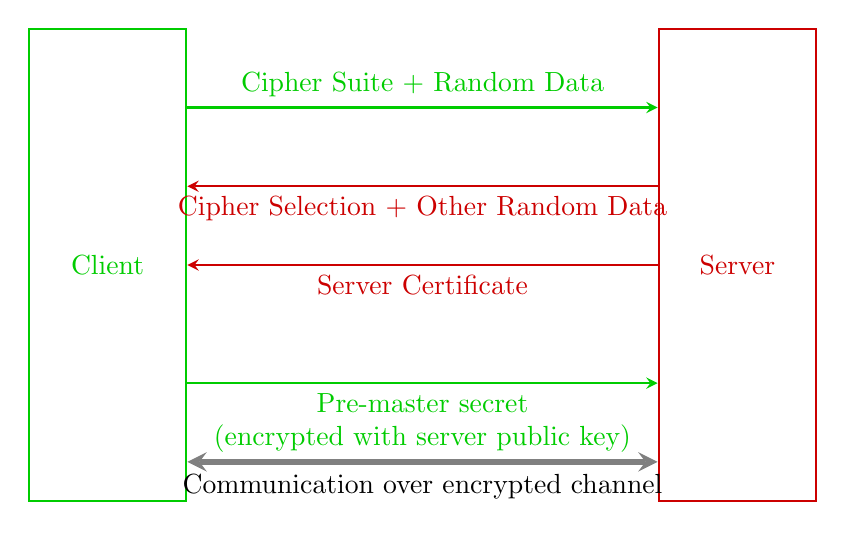
\begin{tikzpicture}[>=stealth, auto, node distance=5cm, thick]
        % Nodes
        \node[draw, green!80!black, minimum width=2cm, minimum height=6cm] (client) {Client};
        \node[draw, red!80!black, minimum width=2cm, minimum height=6cm, right of=client, node distance=8cm] (server) {Server};

        % Phase 1: Hello
        \draw[->, green!80!black] ([yshift=2cm]client.east) -- node[above] {Cipher Suite + Random Data} ([yshift=2cm]server.west);
        
        % Phase 2: Server response & Auth
        \draw[<-, red!80!black] ([yshift=1cm]client.east) -- node[below] {Cipher Selection + Other Random Data} ([yshift=1cm]server.west);
        \draw[<-, red!80!black] ([yshift=0cm]client.east) -- node[below] {Server Certificate} ([yshift=0cm]server.west);
        
        % Phase 3: Secret Transmission
        \draw[->, green!80!black] ([yshift=-1.5cm]client.east) -- node[below, align=center] {Pre-master secret \\ (encrypted with server public key)} ([yshift=-1.5cm]server.west);
        
        % Phase 4: Encrypted channel
        \draw[<->, gray, line width=2pt] ([yshift=-2.5cm]client.east) -- node[below, text=black] {Communication over encrypted channel} ([yshift=-2.5cm]server.west);
        
    \end{tikzpicture}
    \caption{Simplified TLS Handshake flow.}
    \label{fig:tls_handshake}
\end{figure}

\begin{enumerate}
    \item \textbf{Hello Phase:} The client sends the supported cipher suites and some random data. The server responds with the selected cipher suite and its own random data.
    \item \textbf{Server Authentication:} The server sends its X.509 digital certificate to the client. The client must verify this certificate:
    \begin{itemize}
        \item Is it within its validity period?
        \item Is the root Certificate Authority (CA) trusted by the OS/browser?
        \item Is the certificate mathematically valid (signature check)?
        \item Is it revoked (via CRL or OCSP)?
        \item Is the Common Name (or Subject Alternative Name) in the certificate exactly matching the requested domain?
    \end{itemize}
    
    \begin{tcolorbox}[colback=blue!5!white,colframe=blue!75!black,title=Exam Insight]
    Questions about this topic often involve analyzing PKI and Certificate practices. You might be asked to evaluate certificate validation steps, analyze different PKI architectures (e.g., graph vs. tree structures, mechanisms for air-gapped devices), or discuss the security implications of certificate lifetime reduction. Be prepared to explain how each step of validation prevents specific impersonation or MITM attacks.
    \end{tcolorbox}

    \item \textbf{Secret Transmission:} The client generates a \textit{pre-master secret}, encrypts it with the server's public key (extracted from the certificate), and sends it to the server. Only the legitimate server possessing the corresponding private key can decrypt this message.
    \item \textbf{Client Authentication (Optional):} If requested by the server, the client can also send its own certificate and prove possession of the private key by signing a piece of data (usually a hash of the previous handshake messages).
    \item \textbf{Secret Computation:} Both parties now independently compute the \textit{shared secret} (master secret) using the pre-master secret, the client's random data, and the server's random data.
    \item \textbf{Encrypted Communication Phase:} All subsequent communication is symmetrically encrypted and integrity-protected using keys derived from the shared master secret.
\end{enumerate}

\subsection{Resistance to Man-In-The-Middle (MITM) Attacks}
TLS is resistant to MITM attacks by design. Let's analyze what an attacker in the middle could attempt:
\begin{itemize}
    \item \textbf{Let the original certificate through:} The MITM intercepts the traffic but cannot decrypt the pre-master secret because they do not possess the server's private key. They can see the encrypted traffic but lack the shared master key.
    \item \textbf{Send a fake certificate (signed by a non-trusted CA):} The client's browser will reject it because the CA is not in its trusted root store.
    \item \textbf{Send a good certificate with a fake name:} The client will reject it because the requested domain name will not match the certificate's subject name.
    \item \textbf{Send a good certificate but substitute the public key:} This invalidates the CA's digital signature on the certificate, causing the client to reject it.
\end{itemize}

\subsection{TLS Pros and Cons}
\textbf{Pros:}
\begin{itemize}
    \item Protects transmissions (Confidentiality, Integrity).
    \item Ensures authentication of the server, and optionally the client.
\end{itemize}
\textbf{Cons:}
\begin{itemize}
    \item No protection before or after transmission: the data is plaintext on the server and on the client. A trojan on the client or a malicious merchant can still abuse the data.
    \item Relies heavily on the Public Key Infrastructure (PKI).
    \item It is not foolproof, especially regarding user interface and human factors.
\end{itemize}

\section{Security UI and SSL Stripping}
While the cryptographic protocol is secure, the user interface and human gullibility introduce vulnerabilities. 

\subsection{Social Engineering and Warnings}
In early browsers, invalid certificates resulted in a simple dialog box prompting the user ``Do you want to proceed? (Yes/No)''. Most users reflexively clicked ``Yes'' to access the content, entirely violating the assumptions of TLS and making MITM attacks successful. Modern browsers have evolved their UI to make bypassing security warnings much more difficult and scary, strongly advising users to ``Go Back''.

\subsection{SSL Stripping}
A classic attack is SSL Stripping. A victim attempts to connect to a website via plain HTTP (e.g., typing \texttt{bank.com} instead of \texttt{https://bank.com}). The MITM intercepts this HTTP request, establishes an HTTPS connection with the real server, but serves the victim a plain HTTP version of the site (or a fake login form posting to an HTTP endpoint). The user sees a normal page, unaware that the padlock is missing, and inputs their credentials.

\begin{tcolorbox}[colback=blue!5!white,colframe=blue!75!black,title=Exam Insight]
Questions about this topic usually ask you to propose network mitigations or topology changes to prevent specific attacks. You should be able to suggest protocols (such as VPN, HTTPS/HSTS, IPsec) or configurations (DMZ, NAT, Port Security) and evaluate the effectiveness of these countermeasures in defending against MITM, eavesdropping, and session hijacking after network changes have been made.
\end{tcolorbox}

\section{Overcoming TLS/PKI Limitations}
The security guarantees of TLS depend entirely on the security and trust of the root and intermediate CAs. CAs can generate certificates for any domain, and browsers inherently trust hundreds of CAs pre-installed by the OS or the browser vendor.

\subsection{CA Incidents}
History is rife with CA compromises and mis-issuances:
\begin{itemize}
    \item \textbf{2011 Diginotar:} Compromised, leading to rogue certificates for major domains (distrusted and collapsed).
    \item \textbf{2009-2015 Symantec:} Issued test certificates for existing domains like Google. Caught through CT logs, eventually distrusted.
    \item \textbf{2012 Trustwave:} Issued a MITM certificate for a corporate data loss prevention appliance.
\end{itemize}
Dropping a non-compliant CA is difficult because it instantly breaks access to thousands of legitimate websites using that CA.

\subsection{Defense Mechanisms}
To counter these systemic PKI weaknesses and attacks like SSL stripping, several mechanisms were introduced:

\begin{itemize}
    \item \textbf{HSTS (HTTP Strict Transport Security):} An HTTP header that tells the browser to \textit{always} connect to that domain using HTTPS. Browsers also implement an HSTS preload list, meaning the browser will outright refuse to load certain sites over plain HTTP even on the first visit. This effectively kills SSL stripping.
    \item \textbf{HPKP (HTTP Public Key Pinning):} An HTTP header that told the browser to ``pin'' a specific certificate or CA for a domain. If the site later presented a certificate from a different CA, the browser would refuse it. This defended against CA mis-issuance. However, it was \textbf{deprecated} because a simple configuration error (or a malicious ransom attack pinning an attacker's key) could render a website permanently inaccessible to its users.
    \item \textbf{Certificate Transparency (CT):} CAs must submit the metadata of every issued certificate to an independent, publicly auditable, append-only log. Browsers can enforce this by refusing certificates that lack proof of inclusion in a CT log. This allows site owners to monitor the logs (e.g., via \texttt{https://crt.sh}) and detect if any CA fraudulently issues a certificate for their domain.
\end{itemize}

\section{SET (Secure Electronic Transaction)}

\begin{tcolorbox}[colback=blue!5!white,colframe=blue!75!black,title=Exam Insight]
While SET is a legacy protocol, understanding its cryptographic protocol design (such as the dual signature) is highly relevant for exercises that ask you to analyze, prove the security/integrity of, or design custom secure cryptographic protocols. You may be asked to find vulnerabilities, propose fixes, or design protocols for confidentiality and integrity in specific scenarios (e.g., firmware updates, digitally controlled safes). Understanding how SET separates information without compromising integrity is a key pattern to study.
\end{tcolorbox}

Introduced by a joint effort from the VISA and MasterCard consortium, SET aimed to protect \textit{transactions}, not just connections. 

\subsection{The Approach}
In a standard HTTPS transaction, the user sends their credit card details directly to the merchant, who then forwards them to the payment gateway. The merchant sees the card details, creating a risk.
In SET, the cardholder sends:
\begin{itemize}
    \item The \textbf{order of goods} to the \textbf{merchant} only.
    \item The \textbf{payment data} to the \textbf{payment gateway} only.
\end{itemize}
The gateway is empowered to verify the correspondence between the order and the payment without revealing the card details to the merchant.

\subsection{Dual Signature}
SET uses the concept of a \textit{dual signature} to link two messages intended for two different recipients.

\begin{figure}[htpb]
    \centering
    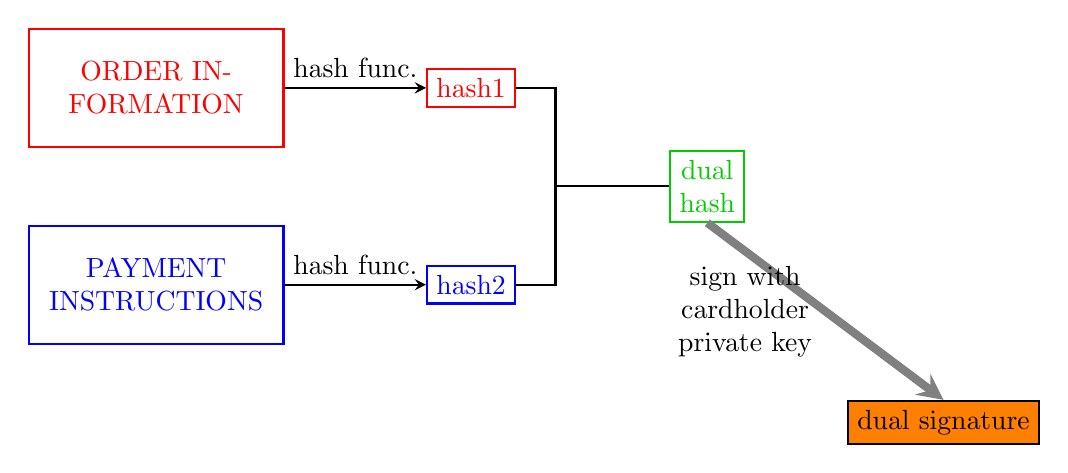
\begin{tikzpicture}[>=stealth, auto, node distance=2.5cm, thick]
        % Nodes
        \node[draw, red, text width=3cm, align=center, minimum height=1.5cm] (order) {ORDER INFORMATION};
        \node[draw, blue, text width=3cm, align=center, minimum height=1.5cm, below of=order] (payment) {PAYMENT INSTRUCTIONS};
        
        \node[draw, red, right of=order, node distance=4cm] (hash1) {hash1};
        \node[draw, blue, right of=payment, node distance=4cm] (hash2) {hash2};
        
        \node[draw, green!80!black, right of=hash1, yshift=-1.25cm, node distance=3cm, align=center] (dualhash) {dual\\hash};
        
        \node[draw, fill=orange, right of=dualhash, node distance=3cm, yshift=-3cm, align=center] (dualsig) {dual signature};

        % Edges
        \draw[->] (order) -- node[above] {hash func.} (hash1);
        \draw[->] (payment) -- node[above] {hash func.} (hash2);
        
        \draw[-] (hash1.east) -- ++(0.5,0) |- (dualhash.west);
        \draw[-] (hash2.east) -- ++(0.5,0) |- (dualhash.west);
        
        \draw[->, gray, line width=3pt] (dualhash.south) -- node[left, text=black, align=center] {sign with \\ cardholder \\ private key} (dualsig.north);
    \end{tikzpicture}
    \caption{Dual Signature Generation in SET.}
    \label{fig:dual_signature}
\end{figure}

The cardholder hashes the order information (\texttt{hash1}) and hashes the payment instructions (\texttt{hash2}). These two hashes are concatenated and hashed again to produce the \texttt{dual hash}. The cardholder then signs this \texttt{dual hash} with their private key, creating the \textit{dual signature}.

\subsection{Data Transmission and Verification}
The cardholder encrypts the order info, \texttt{hash2}, and the dual signature with the merchant's public key. Separately, they encrypt the payment instructions, \texttt{hash1}, and the dual signature with the payment gateway's public key.
\begin{itemize}
    \item \textbf{Merchant side verification:} The merchant decrypts their package, verifies the order, hashes the order info to recreate \texttt{hash1}. They then combine it with the provided \texttt{hash2} to compute the dual hash. Finally, they verify the dual signature using the cardholder's public key.
    \item \textbf{Payment gateway side verification:} The gateway does the perfect dual. It decrypts its package, hashes the payment instructions to recreate \texttt{hash2}, combines it with the provided \texttt{hash1}, computes the dual hash, and verifies the signature.
\end{itemize}

\subsection{Why did SET Fail?}
Despite its elegant cryptographic design, SET failed commercially. 
SET required a digital certificate from all three parties: the Merchant, the Payment Gateway, and the Cardholder. While issuing certificates to merchants and gateways is feasible, requiring every individual consumer to obtain, manage, and use a digital certificate simply \textbf{does not scale}. 
It required a cumbersome pre-registration process for the cardholder. This lack of transparency and steep learning curve meant it never reached critical mass. If a user had to go through a complex setup just to buy a book, they would abandon the purchase.
Nowadays, a simple HTTPS redirect to a bank's tokenized portal is commonly used, providing a transparent and secure user experience without the need for client-side PKI.

\section*{Chapter Summary}
This chapter explores the challenges of securing communications over the Internet, focusing on two major protocols: TLS (Transport Layer Security) and SET (Secure Electronic Transaction). It covers the mechanisms of the TLS handshake, its reliance on Public Key Infrastructure (PKI), and defense mechanisms against attacks like SSL Stripping (e.g., HSTS, Certificate Transparency). Furthermore, it discusses the SET protocol, its innovative use of dual signatures to separate order and payment information, and the reasons for its eventual commercial failure.

\begin{table}[htpb]
    \centering
    \renewcommand{\arraystretch}{1.3}
    \begin{tabular}{|l|p{10cm}|}
        \hline
        \textbf{Protocol} & \textbf{Key Characteristics} \\ \hline
        \textbf{TLS} & Evolved from SSL; provides confidentiality, integrity, and authentication; relies on PKI; vulnerable to CA compromises but mitigated by HSTS and CT. \\ \hline
        \textbf{SET} & Protects transactions rather than just connections; uses dual signatures; failed commercially due to poor scalability and lack of user transparency. \\ \hline
    \end{tabular}
    \caption{Comparison of Network Security Protocols}
    \label{tab:protocol_summary}
\end{table}
